\documentclass[12pt, a4paper, twoside]{article}

%% Preamble
\usepackage{umatfgspanish} % Estilo de la Universidad de Málaga
\usepackage[backend=biber]{biblatex} % Para la bibliografía
\addbibresource{bibliografia.bib} 
\usepackage{subfiles} % Best loaded last in the preamble
\usepackage{blindtext} % Para texto de relleno
\usepackage{verbatim} % Para comentarios
\usepackage{forest} % Para árboles
\usepackage{enumitem} % Para listas con símbolos personalizados
\usepackage{hyperref} % Para enlaces
\usetikzlibrary{arrows.meta}
\graphicspath{ {./images/} }



\begin{document}


%% Front Cover
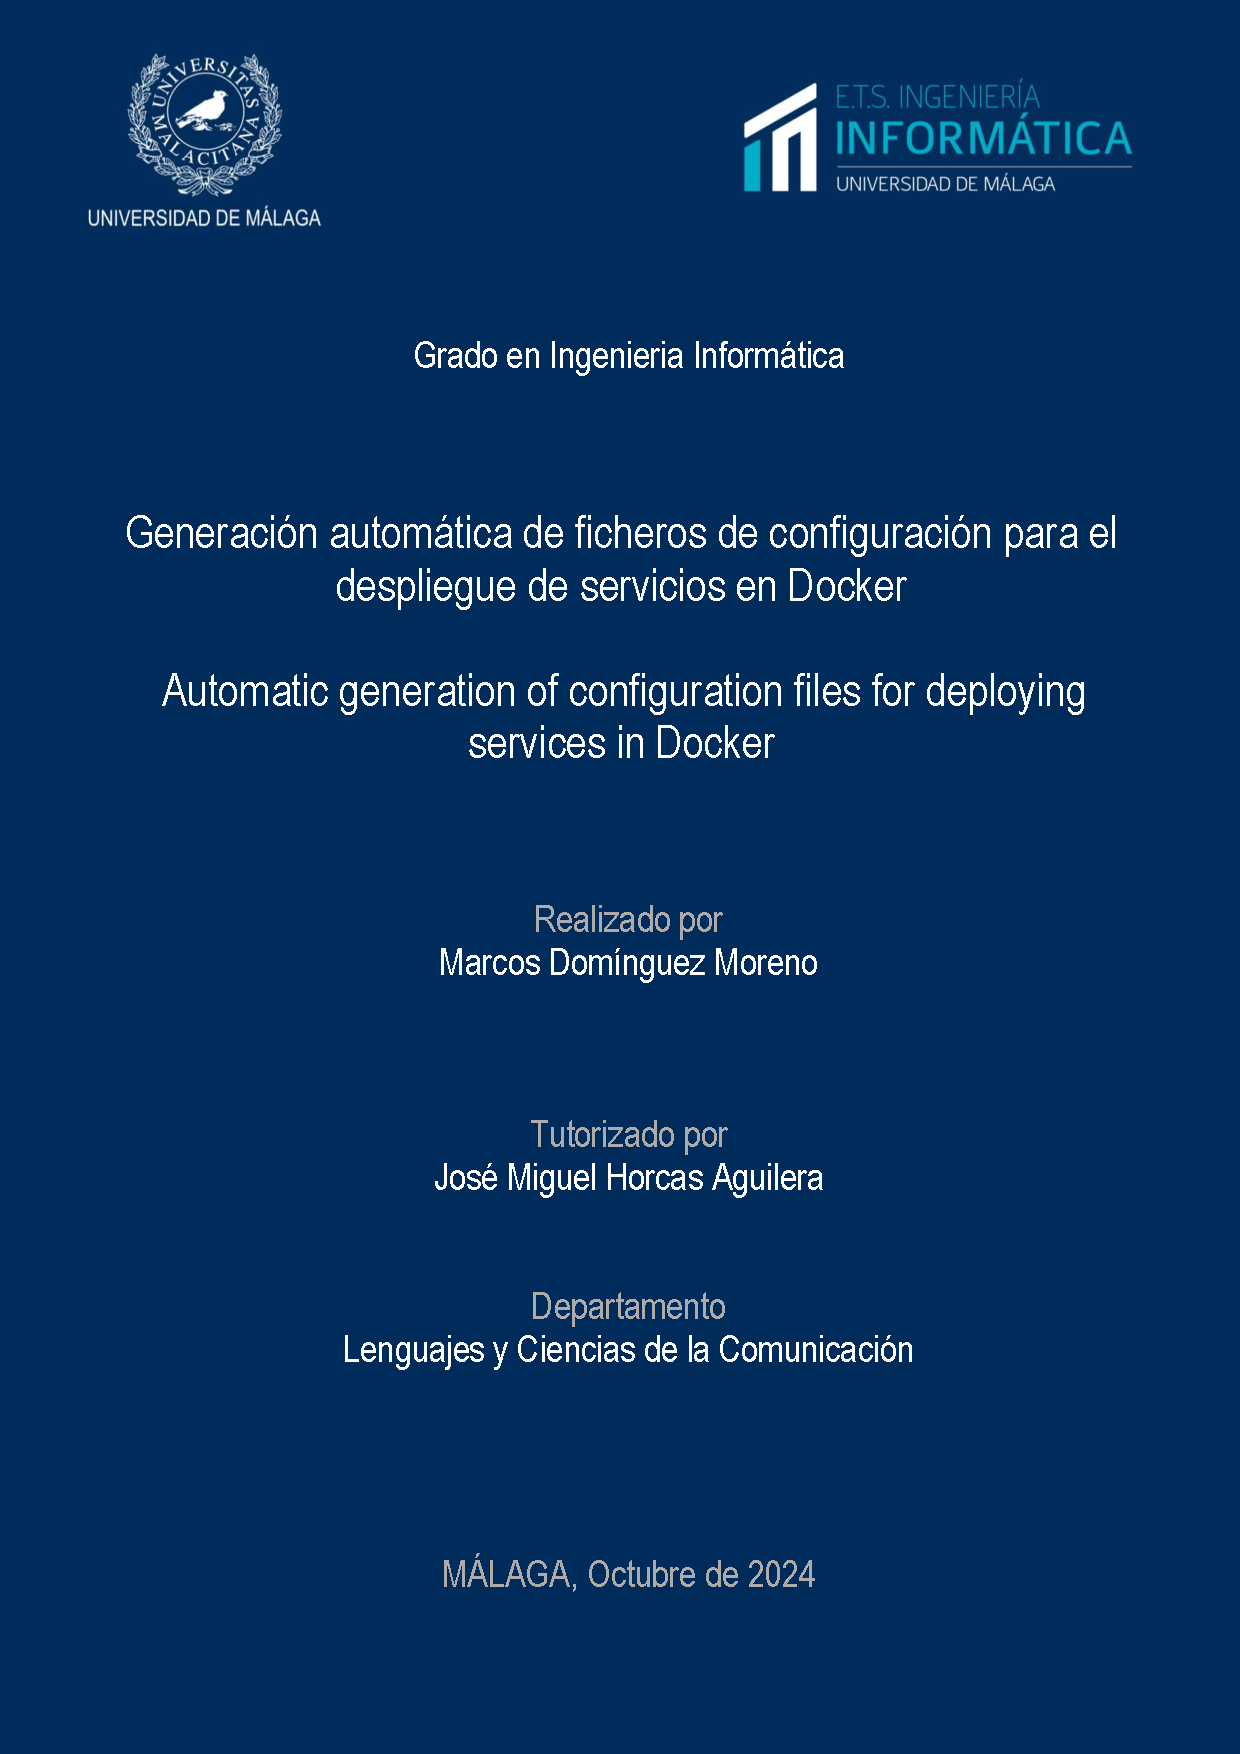
\includepdf[noautoscale=true, width=\paperwidth]{Portada-Titulo-Contraportada/cover.pdf}
\newpage

%% Title Page

\includepdf[noautoscale=true, width=\paperwidth]{Portada-Titulo-Contraportada/title.pdf}

%% Abstract
\subfile{sections/abstract}
\newpage

%% Resumen
\subfile{sections/resumen}
\newpage

% Table of Contents
\tableofcontents
\newpage








%% Introduccion
\section{Introduccion}
\label{sec:Introduccion}

\subsection{Motivación}
Las herramientas de automatización de tareas son fundamentales para la productividad en el desarrollo de software, permiten mejorar la eficiencia, la calidad y la consistencia en la producción de código.
Al relegar tareas repetitivas y propensas a errores a herramientas automatizadas, los desarrolladores pueden centrarse en tareas más creativas y de mayor valor añadido.

Parte del ciclo de vida en un desarrollo de software implica la configuración y el despliegue de servicios en entornos de producción y desarrollo.
La configuracion y despliegue requiere de la creación de archivos de configuración específicos, como son por ejemplo los archivos dockerfile \footnote{\hyperref[sec:Dockerfile]{Dockerfile}} y .dockerignore \footnote{\hyperref[sec:dockerignore]{dockerignore}}, que definen cómo se construye la imagen de un contenedor en tecnologicas como Docker \footnote{ \hyperref[sec:Docker]{Docker}}

En el contexto de la tecnología de contenedores, Docker se ha convertido en una de las plataformas más populares para la creación, el despliegue y la gestión de aplicaciones en entornos contenerizados. 
Sin embargo, la configuración de servicios en Docker puede ser una tarea compleja y propensa a errores, especialmente cuando se manejan múltiples servicios y configuraciones.

La motivación para realizar este proyecto surge de la necesidad de simplificar y automatizar el proceso de generación de archivos de configuración para el despliegue de servicios en Docker. 
En la actualidad, la creación manual de estos archivos dockerfile puede ser una tarea repetitiva y susceptible a fallos al no conocer el usuario de toda la informacion necesaria para la correcta configuracion de los servicios, 

Al desarrollar una herramienta que automatice este proceso, 
se busca mejorar la eficiencia y la precisión en la configuración de entornos de contenedores, facilitando así el trabajo de desarrollo y administracion. 

\subsection{Objetivo}
La meta principal de este proyecto es desarrollar una herramienta que permita la generación automática de archivos de configuración para el despliegue de servicios en Docker.
Siguiendo las pautas recomendadas para la generacion de dichos archivos mediante de plantillas, las plantillas han de ser extensibles y adaptables a los cambios en un futuro sin necesidad de reescribir código.
\\ \\
Para ello se plantean los siguientes objetivos específicos:
\begin{itemize}
	\item Investigar y analizar las tecnologías y herramientas existentes para la generación de archivos de configuración en Docker.
	\item Desarrollar una plantilla orientada a la generacion de ficheros dockerfile siguiendo las buenas practicas.
	\item Implementar un modelo de plantillas extensible y adaptable a los cambios en las tecnologías y las metodologías de desarrollo.
	\item Desarrollar una herramienta web que permita la selección de plantillas y la generación de archivos de configuración para el despliegue de servicios en Docker.
	\item Desplegar la aplicación en un entorno no orientado a producción y documentar el proceso de instalación y uso.
	\item Evaluar la eficacia y la usabilidad de la herramienta en la memoria.
\end{itemize}

\newpage 
\subsection{Resultados Esperados}
Dada la gran cantidad de opciones de configuración disponibles en para la generacion de ficheros de configuracion, el desarrollo de esta herramienta presenta varios desafíos técnicos y conceptuales.
El primero de ellos es la magnitud de las opciones de configuración disponibles, que pueden variar en función de las necesidades y los requisitos de cada servicio.
dar una covertura a todos los escenarios posibles es una tarea inabarcable, por lo que se ha optado por centrarse en los casos de uso más comunes y en las configuraciones más utilizadas en la práctica.
Sin embargo se espera que la herramienta sea lo suficientemente flexible y extensible como para permitir la incorporación de nuevas plantillas y configuraciones en el futuro.

Los desarrollos de los servicios resultantes de la implementacion no tendran el objetivo de alcanzar un estado de produccion sino de servir como base para futuras implementaciones y desarrollos orientados a ello 

\subsection{Estructura del documento}

\begin{itemize}[label=\textbullet]
	\item El \hyperref[sec:Introduccion]{Capitulo 1 } describe la motivación del trabajo, sus objetivos, y los resultados esperados.
	\item El \hyperref[sec:Estado del Arte]{Capitulo 2 } presenta una brebe introduccion a los contenidos, al estado del arte, soluciones existentes y que se aporta en este contexto.
	\item El \hyperref[sec:Tecnologias Empleadas]{Capitulo 3 } describe las tecnologías y herramientas empleadas en el desarrollo del proyecto.
	\item El \hyperref[sec:Metodologia]{Capitulo 4 } describe la metodología de trabajo empleada en el desarrollo del proyecto.
	\item El \hyperref[sec:Modelado de las plantillas]{Capitulo 5 } describe el modelado de las plantillas.
	\item El \hyperref[sec:Arquitectura y Descripcion del sistema]{Capitulo 6 } describe la arquitectura del proyecto y junto con la descripcion de los servicios
	\item El \hyperref[sec:Extensibilidad]{Capitulo 7 } es un capitulo dedicado a la extensibilidad de las plantillas
	\item El \hyperref[sec:Despliegue de la aplicación]{Capitulo 8 }  describe el despliegue de la aplicación en un entorno no orientado a producción.
	\item El \hyperref[sec:Resultados]{Capitulo 9 } presenta los resultados obtenidos en el desarrollo del proyecto.
	\item El \hyperref[sec:Conclusiones]{Capitulo 10 } incluye las conclusiones del trabajo y las recomendaciones para trabajos futuros.
	\item El \hyperref[sec:Manual de Instalación]{Apendice A} Es un manual de Instalacion de la aplicacion
	\item El \hyperref[sec:Manual de Uso]{Apendice B} Es un manual de Uso de la aplicacion
	\item El \hyperref[sec:Manual de Desarrollo]{Apendice C} Es una guia para el desarrollo de plantillas.
\end{itemize}















%% Estado del Arte 
\section{Estado del Arte}
\label{sec:Estado del Arte}
Para comprender el sentido de este proyecto y su problematica es necesario contextualizar algunos conceptos previos que son necesarios para comprender la situacion actual y contextualizar la problematica.
A continuacion se introducen dichos conceptos de manera escalonada, abordaremos la problematica de la generacion de archivos de configuracion en Docker, las tecnologias empleadas en la generacion de dichos archivos y las soluciones actualmente disponibles.

\subsection{Contenedores}
Los contenedores son paquetes software ligeros que incluyen el código de las aplicaciones junto con sus dependencias, como versiones concretas de entornos de ejecución de ciertos lenguajes de programación y bibliotecas para ejecutar los servicios de software. \cite{googlecontainers}
\subsubsection{Porque se usan los contenedores}
Los contenedores constituyen un mecanismo de empaquetado lógico en el que las aplicaciones pueden extraerse del entorno en que realmente se ejecutan. 
Esta desvinculación facilita el despliegue uniforme de las aplicaciones basadas en ellos con independencia de que el entorno sea un centro de datos privado, la nube pública o el portátil personal de un desarrollador. \cite{googlecontainers}
Es una solucion de facil aplicacion, alto rendimiento y extremadamente portable. \footnote{Existen restricciones en cuanto a la portabilidad de los contenedores, pero en general son facilmente desplegables en cualquier entorno enlace:\href{https://stackoverflow.com/questions/42158596/can-windows-containers-be-hosted-on-linux}{https://stackoverflow.com/questions/42158596/can-windows-containers-be-hosted-on-linux}}
\newpage

\subsection{Imagenes}
Las imágenes de contenedores son plantillas de solo lectura que contienen el código de la aplicación, las bibliotecas, las dependencias y otros archivos necesarios para ejecutar un contenedor. \cite{awsdocker} 
No necesariamente necestiamos de una imagen para construir un contenedor \footnote{Existe la posbilidad de crear contenedores de otras formas como a partir de otros contenedores} pero ese es el escenario más común. \footnote{contruir un contenedor a partir de una imagen lo hace reproducible}
\subsection{Docker}
\label{sec:Docker}
Docker \cite{docker} es un proyecto de código abierto que automatiza el despliegue de aplicaciones dentro de contenedores de software, proporcionando una capa adicional de abstracción y automatización de virtualización de aplicaciones en múltiples sistemas operativos
Docker es una plataforma de código abierto que permite a los desarrolladores crear, desplegar y ejecutar aplicaciones en contenedores. 
\footnote{Existen alternativas a Docker como Podman \cite{podman} pero Docker es la más popular y ampliamente utilizada en la actualidad.}
\subsubsection{Dockerfile}
\label{sec:Dockerfile}
El archivo Dockerfile \cite{dockerfile_concepts} es un archivo de texto que contiene una serie de instrucciones que Docker utilizará para construir una imagen de contenedor.
Usualmente la construccion de un archivo de configuracion se realiza a partir de una imagen base, que puede ser una imagen oficial de Docker o una imagen personalizada creada por el usuario.
A dicha imagen se añaden las instrucciones necesarias para instalar las dependencias y configurar el entorno de ejecución de la aplicación, lo que viene a representar el contenido de un archivo Dockerfile.
\subsubsection{dockerignore}
\label{sec:dockerignore}
El fichero .dockerignore \cite{dockerignore} es un tipo de archivo que puede colocarse en el proyecto del usuario y que se utiliza con la función de ignorar ficheros y directorios durante el docker build, con el objetivo de evitar que estos se copien a la imagen de Docker 
\newpage
\subsubsection{Buenas Prácticas en la creacion de las imagenes}
Para la creacion de los ficheros dockerfile es recomendable seguir una serie de buenas practicas para garantizar la eficiencia y la seguridad en el despliegue de servicios en Docker.
Estas practicas se recojen en la documentacion oficial de Docker \cite{dockerfile_best_practices}
En la documentacion se abordan una serie de recomendaciones para la creacion de imagenes de contenedores en Docker, entre las que se incluyen:
\begin{itemize}
    \item Utilizar imágenes oficiales de Docker:
    \begin{itemize}
        \item Las imágenes oficiales son mantenidas y actualizadas por la comunidad de Docker, lo que garantiza un alto nivel de seguridad y estabilidad.
        \item Estas imágenes suelen estar optimizadas para un rendimiento eficiente y son ampliamente documentadas.
    \end{itemize}
    
    \item Crea ficheros de configuracion dockerfile Multietapa:
    \begin{itemize}
        \item Crear imágenes en varias etapas permiten dividir la construcción de la imagen, lo que puede mejorar el rendimiento
        \item Esto ayuda a reducir el tamaño final de la imagen al incluir solo los archivos necesarios para la ejecución de la aplicación.
    \end{itemize}
    
    \item Usar una imagen base ligera:
    \begin{itemize}
        \item Utilizar imágenes base ligeras, como `alpine`, puede reducir significativamente el tamaño de la imagen Docker.
        \item Las imágenes ligeras también suelen tener menos vulnerabilidades de seguridad debido a su menor superficie de ataque.
    \end{itemize}
    
    \item Reducir el número de capas:
    \begin{itemize}
        \item Cada instrucción en un Dockerfile crea una nueva capa en la imagen. Reducir el número de capas puede mejorar el rendimiento y reducir el tamaño de la imagen.
        \item Combinar múltiples comandos en una sola instrucción `RUN` puede ayudar a minimizar el número de capas.
    \end{itemize}
    
    \item Eliminar archivos innecesarios:
    \begin{itemize}
        \item Durante el proceso de construcción, es importante eliminar cualquier archivo temporal o innecesario para mantener la imagen lo más pequeña posible.
    \end{itemize}
    
    \item Evitar el uso de la etiqueta `latest`:
    \begin{itemize}
        \item La etiqueta `latest` puede ser ambigua y llevar a problemas de consistencia y reproducibilidad.
        \item Es mejor especificar una versión concreta de la imagen para asegurar que se está utilizando la versión correcta.
    \end{itemize}
    
    \item Eliminar archivos temporales y de instalación:
    \begin{itemize}
        \item Durante la instalación de paquetes y dependencias, se generan archivos temporales que deben ser eliminados para reducir el tamaño de la imagen.
        \item Utilizar comandos como `apt-get clean` y `rm -rf /var/lib/apt/lists/*` para limpiar los archivos de instalación.
    \end{itemize}
    

    
\end{itemize}
\footnote{ Para más informacion: \href{https://docs.docker.com/build/building/best-practices/}{https://docs.docker.com/build/building/best-practices/}}
\newpage 

\subsection{Problematica}
La dificultad de crear imagenes reside en la naturaleza de la aplicacion que queremos llevar a un contenedor, existen una gran cantidad de escenarios donde si bien la tarea es sencilla, esta puede escoder una complejidad implicita
de la que el usuario no es consciente. 
Estos apartados repercuten en el tiempo de compilación, tamaño de la imagen, mantenibilidad, seguridad y repetibilidad en las imagenes que se crean. \\
La calidad de las imagenes pueden marcan una diferencia que puede llegar a ser crítica para posteriores etapas en el desarrollo de aplicaciones como son la Orquestacion de contenedores \cite{ibm_container_orchestration}.

\subsection{Soluciones Actualmente Disponibles}
En la actualidad hay disponibles varias soluciones para disminuir la complejidad implicita que reside en en la configuracion de dichos ficheros dockerfile. Existen más herramientas que las representadas a continuacion pero estas son las más empleadas.
\subsubsection{Docker init}
Docker init es el comando de Docker Desktop \cite{docker_desktop} que permite inicializar un proyecto con un archivo de configuración básico.
su funcionamiento consta de elegir una plantilla de proyecto y seleccionar entre las opciones de configuracion.
Las opciones de configuracion se limitan a elegir el lenguaje de programacion, puerto en el que despliega la aplicacion y que comando se ejecutara al iniciar el contenedor.
Las plantillas son creadas y mantenidas por la comunidad \footnote{En este proyecto se reutilizan y se recogen ideas de varias de las plantillas que incluye Docker Init}
\begin{figure}[ht]
  \centering
    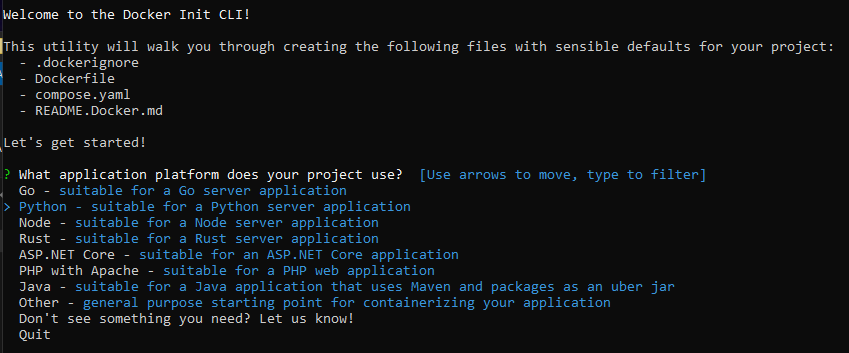
\includegraphics[width=1\textwidth]{Docker Init.png}
  \caption{Captura de las opciones de Plantillas disponibles Docker Init.}
\end{figure}

\newpage
\subsubsection{Docker Extension for Visual Studio Code}
La extension de Docker para visual estudio code \cite{vscode_containers_overview} permite entre otras muchas de sus funcionalidades la generacion del fichero dockerfile entre otros.
su comportamineto es similar al de Docker init, permitiendo entre otras opciones elegir el lenguaje de desarrollo del proyecto y que comando se ejecutara al iniciar el contenedor.

\begin{figure}[ht]
	\centering
	  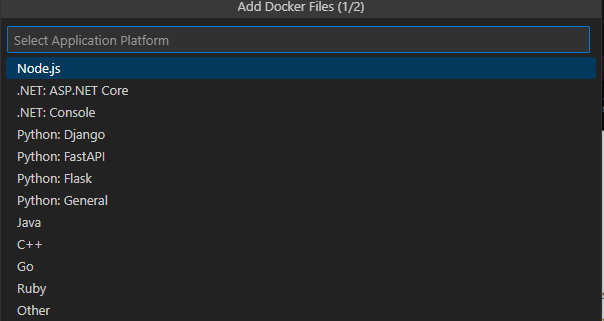
\includegraphics[width=1\textwidth]{Docker.extension.vscode.png}
	\caption{Plantillas Disponibles en la Extesnsion para Docker de Visual Studio Code.}
\end{figure}

\begin{figure}[ht]
	\centering
		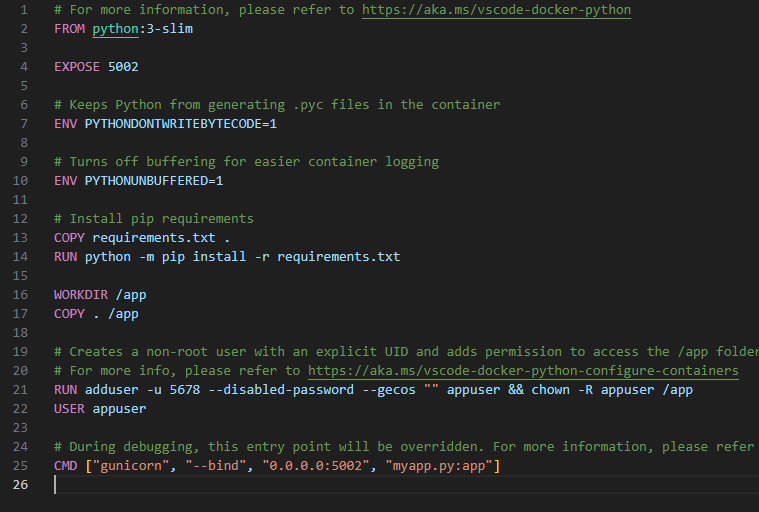
\includegraphics[width=1\textwidth]{docker.extension.vscode.dockerfile.png}
	\caption{Captura de una plantilla generada por la Extesion para Docker de Visual Studio Code}
\end{figure}

\subsubsection{Inteligencia Artificial}
En la actualidad existen soluciones que se apoyan en la inteligacia Artificial para la generacion de archivos de configuracion, y para la creacion de los fichero dockerfile. 
La calidad de estas soluciones es variable y depende de la calidad de los modelos de lenguaje natural empleados y de la calidad del prompt\footnote{Instrucción o texto inicial proporcionado a una herramienta generativa de IA para dirigir la generación de respuestas o resultados específicos \cite{panamericanlatam_prompt_ia}} de entrada.
como magickpen \cite{magickpen_dockerfile_template} \footnote{\href{https://magickpen.com/templates/128/}{magickpen:https://magickpen.com/templates/128/}} o alternativas con propositito más general como chatgpt \cite{chatgpt} \footnote{\href{https://chat.openai.com/}{chatgpt:https://chat.openai.com/}}

\begin{figure}[ht]
	\centering
		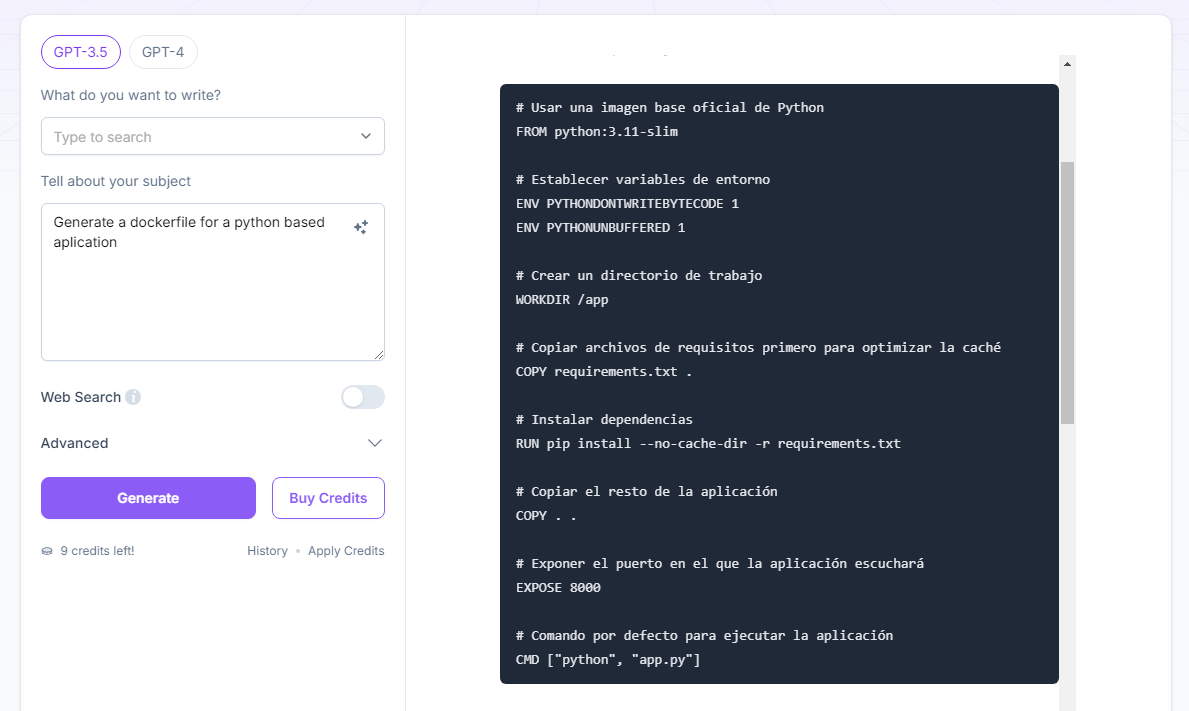
\includegraphics[width=1\textwidth]{MagickPen.png}
	\caption{Captura de un resultado de magickpen}
\end{figure}


\newpage
\subsection{Conclusiones Preliminares}
En este estudio se han recogido algunas de las principales herramientas y tecnologías disponibles en la actualidad para la generación de archivos de configuración.
Todas las herraminetas (Salvo propiamente los Modelos de Texto Generativo) hacen uso de plantillas para la generacion de los ficheros dockerfile y dockerignore, estas plantillas si bien son correctas son por naturaleza limitadas y no permiten la personalizacion más final de las opciones de configuracion.
No obstante suponen un punto de partida para el desarrollo de aplicaiones 

\subsection{Que se aporta en este contexto:}
Las opciones actualemtne disponibles para la generacion de archivos de configuracion para el despliegue de servicios en Docker son limitadas y no permiten la personalizacion de las opciones de configuracion.
Se deja de lado la variabilidad y las posibles opciones que existen a la hora de construir las imagenes, el proyecto proporcinara una nueva forma de construir plantillas dotando capacidad al usuario de una personalizacion
más profunda y detallada de las opciones de configuracion de los servicios en Docker.
\subsubsection{Software Product Line SPL}
El proyecto propone una solucion en linea con la implementacion de plantillas pero enfocando estas plantillas como si formaran parte de una linea de productos software.
Una línea de productos software (SPL del inglés Software Product Line) es una familia de productos software 
relacionados entre sí que comparten ciertas características comunes (similitudes) pero que también tienen 
características variables. CITA Documentacion

En un SPL, los sistemas se descomponen en características (features) que representan funcionalidades o comportamientos del sistema. 
El principal artefacto para modelar la variabilidad en SPL son los modelos de variabilidad. Existen muchos modelos 
de variabilidad pero los más extendidos y usados en la práctica son los modelos de características (feature models). 

Un feature model (FM) \cite{wikipedia_feature_model} es un modelo para representar la variabilidad de una SPL en base a características comunes y 
variables (véase Figura 1), especificando qué características se pueden seleccionar en una configuración para generar 
un producto válido de la SPL. CITA 

\begin{figure}[ht]
	\centering
		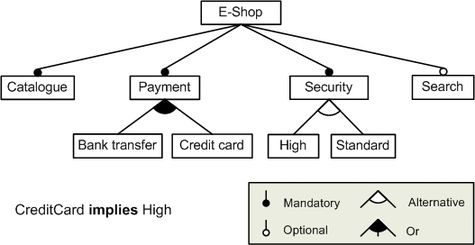
\includegraphics[width=1\textwidth]{fm.example.jpg}
	\caption{Ejemplo Represantcion Grafia de un feature model \cite{wikipedia_feature_model}}
\end{figure}












%% Tecnologías Empleadas
\section{Tecnologías Empleadas}
\label{sec:Tecnologias Empleadas}
Este apartado describe las tecnologías y herramientas empleadas más relevantes para el desarrollo del proyecto, así como su función y su relación con el objetivo del proyecto.

\subsection{Universal Variability Language UVL}

La Universal Variability Language (UVL) \cite{uvl} es un lenguaje de modelado diseñado específicamente para representar y manejar la variabilidad en sistemas software. 
La variabilidad en software se refiere a las partes de un sistema que pueden personalizarse, configurarse o cambiarse para adaptarse a diferentes necesidades o contextos. 
UVL se usa comúnmente en el contexto de ingeniería de líneas de productos de software (Software Product Line Engineering o SPLE), donde se trabaja con una familia de productos que comparten un núcleo común, pero pueden tener variaciones.
todas las plantillas que se han desarrollado en este proyecto requieren de un archivo UVL para poder generar configuraciones validas.

\subsection{Docker}
La apliccion web tanto como todos sus servicios han sido desarrollados con el objetivo en mente de ser ejecutados dentro de contenedores
Para el manejo de los contenedores en el entorno de desarrollo se ha optado por la utilizacion de Docker Desktop es complemento con la consola de comandos.
Esta herremienta ayuda al proyecto en el momento en que lo hacer portable y facil de desplegar en cualquier entorno.
\subsection{Node.js}
\cite{nodejs}
para el desarrollo de la aplicacion web se ha optado por la utilizacion de Node.js como entorno de ejecucion de JavaScript para el desarrollo Frontend.
Esta herramienta constituye una plataforma de desarrollo en tiempo de ejecución cuenta con la ventaja de contar con una extensa biblioteca de módulos que simplifican el desarrollo de aplicaciones web.
Con npm (Node Package Manager) \cite{npm}, Node.js ofrece acceso a una vasta colección de paquetes y módulos que pueden ser fácilmente integrados en el proyecto, acelerando el desarrollo y reduciendo la necesidad de escribir código desde cero.
Para el proyecto se emplea la version v22.10.0 y la version v10.9.0 del gestor de paquetes npm
\subsection{Angular}
\cite{angular}
En cuanto al desarrollo de la aplicacion web se ha optado por la utilizacion de Angular como framework de desarrollo.
El motivo de esta decision es la idea de emplear un framework moderno para emplear los metodos de desarrollo actuales y las mejores practicas en el desarrollo de aplicaciones web.
Emplear otros framework de desarrollo como React o Vue.js tambien hubiera sido una opcion valida al existir una cierta convergencia entre ellos en cuanto a funcionalidades y caracteristicas.
Para los requisitos del proyecto entendimos que Angular ya integra gran parte de las funcionalidades que requesia nuestra aplicacion ahorrando tiempo en la implementacion de las mismas. La version empleada es Angular v18 \footnote{Angular 18 no es la ultima version disponible pero al depender de otros desarrollo se ha optado por la utilizacion de esta version}
\subsubsection{Angular Material}
\cite{angular_material}
Para el diseño de la interfaz grafica de la aplicacion web se ha optado por la utilizacion los componentes provenientes de los modulos de Angular Material.
Siguiendo la linea de diseño de Material Design, Angular Material proporciona una serie de componentes y directivas que facilitan la creacion de interfaces de usuario modernas y atractivas.
Los componentes tienen una reaccion conocidad por el usuario y son faciles de implementar en la aplicacion web. \footnote{La ultima version disponible es 18.2.9 }
\subsubsection{Monaco Editor}
\cite{monaco_editor} Para la edicion de los archivos de configuracion se ha optado por la utilizacion de Monaco Editor como editor de codigo.
Monaco Editor es un editor de codigo fuente basado en la web que se utiliza en varios proyectos de Microsoft, como Visual Studio Code, Azure DevOps y el editor de codigo de GitHub.
cuenta con una serie de caracteristicas que lo hacen ideal para la edicion de archivos de configuracion, como la resaltado de sintaxis, el autocompletado y la verificacion de errores.
tambien es altamente personalizable y extensible, lo que permite adaptarlo a las necesidades del proyecto. \footnote{La ultima version de angular en la que es compatible es la v18 por este motivo se ha desarrollado en esta version de Angular \href{https://www.npmjs.com/package/ngx-monaco-editor-v2}{https://www.npmjs.com/package/ngx-monaco-editor-v2}}
\subsubsection{ngx-json-viewer}
\cite{ngx_json_viewer}
Para la visualizacion de los archivos de configuracion se ha optado por la utilizacion de ngx-json-viewer como visor de archivos json.
ngx-json-viewer es un componente de Angular que permite visualizar archivos JSON en un formato legible y estructurado.
es un proyecto de codigo abierto que se puede integrar facilmente en aplicaciones Angular y personalizar segun las necesidades del proyecto.

\subsection{Nginx}
\cite{nginx} 
Nginx es un servidor web de código abierto desarrollado en C que se utiliza para servir contenido web estático y dinámico, así como para actuar como proxy inverso y balanceador de carga.
la ventaja de Nginx es principalmente la poca necesidad de configuracion que requiere para su correcto funcionamiento, ademas de ser un servidor web ligero y de alto rendimiento.
Para las necesidades del proyecto se ha empleado en sus funciones de proxy inverso para redirigir las peticiones de la aplicacion web al servidor de backend.
y como servidor web para servir el contenido estatico de la aplicacion web.

\subsection{Python}
\cite{python}
Python es un lenguaje de programación de alto nivel, interpretado y de propósito general que se ha convertido en uno de los lenguajes más populares en la actualidad.
Para el desarrollo de los servicios de backend se ha optado por la utilizacion de Python como lenguaje de programacion.
Python es conocido por su sintaxis clara y legible, su amplia biblioteca estándar y su soporte para múltiples paradigmas de programación, como la programación orientada a objetos, la programación funcional y la programación imperativa.
\subsubsection{Flask}
\cite{flask}
Flask es un microframework de Python para el desarrollo de aplicaciones web.
Flask es conocido por su simplicidad y su facilidad de uso, lo que lo convierte en una excelente opción para el desarrollo de aplicaciones web pequeñas y medianas.
\subsubsection{Gunicorn}
\cite{gunicorn}
Gunicorn es un servidor HTTP WSGI para Python que se utiliza para servir aplicaciones web desarrolladas en Python. su objetivo es proporcionar un servidor web simple y eficiente que pueda manejar múltiples solicitudes simultáneamente.
esta herraminta es necesaria para el despliegue de la aplicacion en un entorno de produccion.
\subsubsection{Pypi}
\cite{pypi}
El uso de Pypi como repositorio de paquetes de Python es necesario para la instalacion de las dependencias de la aplicacion.
asi como ha sido empleado para subir paquetes diseñados para la aplicacion.

\subsection{Jinja}
\cite{jinja}
Jinja es un motor de plantillas para Python que se utiliza para generar archivos de texto dinámicos basados en plantillas. 

\subsubsection{Jinja2}
Jinja2 es la versión más reciente de Jinja y se utiliza comúnmente en aplicaciones web de Python para generar contenido dinámico.
Jinja2 es conocido por su sintaxis simple y legible, su capacidad para generar contenido dinámico y su integración con Python y otros marcos de desarrollo web.
Jinja2 permite la generacion de archivos de texto dinamicos basados en plantillas, lo que facilita la creacion de archivos de configuracion personalizados y adaptables a las necesidades del usuario.
Todas las plantillas desarrolladas han usando la sintaxis de Jinja2



\subsection{Git}
\cite{git}
Para el control de versiones se ha optado por la utilizacion de Git como sistema de control de versiones.
\subsection{GitHub}
\cite{github}
GitHub es una plataforma de desarrollo colaborativo que se utiliza para alojar proyectos de código, realizar seguimiento de problemas y tareas, y colaborar con otros desarrolladores.
Todo el proyecto es alojado en GitHub incluyendo plantillas, codigo ...
\subsubsection{GitHub Public Api}
\cite{github_rest_api}
Para la gestion de las plantillas se ha empleado la API publica de GitHub para la obtencion de las plantillas disponibles.
Esta desion se ha tomado por facilidad de uso, ya que la API de GitHub es ampliamente conocida y documentada, y permite acceder a una gran cantidad de información sobre los repositorios y las plantillas disponibles.
Esto supone que las plantillas estan visibles y son accesibles y modificables por cualquier usuario de GitHub.
Simplificando el proceso de creacion, mantenimiento y actualizacion de las plantillas. 

\newpage

\subsection{Visual Studio Code}
\cite{vscode}
Visual Estudio Code es un editor de código fuente desarrollado por Microsoft que se utiliza para escribir, editar y depurar código.
Su mencion se debe a que es el editor de codigo fuente que se ha empleado para el desarrollo del proyecto. Ademas de ser clave en el proceso de generador de ficheros de configuracion
de los que la aplicacion hace uso.
\subsubsection{UVLS extension}
\cite{uvls_code}
UVLS es una extension de Visual Studio Code que proporciona soporte para la Universal Variability Language (UVL) en el editor de codigo.
La extension UVLS proporciona resaltado de sintaxis, autocompletado, verificacion de errores y otras funcionalidades que facilitan la edicion de archivos de configuracion en UVL.
ademas la clave más importante es que es la unica herramienta existente que permite crear una configuracion correcta partiendo desde un Feature Model


Otras extensiones de menos importancia empleadas en \textit{VSCode} son:
\begin{itemize}
    \item \textbf{Docker Extesnion}
    \item \textbf{Flama}
    \item \textbf{Graphviz Interactive Preview}
    \item \textbf{Latex Workshop}
    \item \textbf{Pylance}
    \item \textbf{Python Debugger}
    \item \textbf{Better Jinja}
\end{itemize}










%% Metodología
\section{Metodologia del trabajo}
\label{sec:Metodologia}
\subsection{Introduccion}
El enfoque se ha dado para abordar el desarrollo de este trabajo ha consistido en combinar un trabajo previo de analisis e investigacion con una fase de desarrollo iterativo.
\\La investigacion y analisis tenia el objetivo de conocer en profundidad las tecnologias y herramientas empleadas 
para porstesiromete estudiar una posible aplicacion de estas ideas y conceptos en el desarrollo de las plantillas.
una vez resuelta esta primera parte se ha procedido a una toma de requisitos y a la planificacion de la implementacion de la aplicacion,
para la implementacion de la aplicacion se ha optado por la utilizacion de una metodologia de desarrollo que permita la evolucion del proyecto a un producto minimo viable en el menor tiempo posible.
\subsection{Metodología del Desarrollo}
Para la implementacion del Proyecto se ha optado por un desarrollo en Cascada al tener una idea muy definida de lo que se quiere desarrollar y de las tecnologias empleadas.
Los cambios más relevaten surgen en las plantillas es por ello que contamos con los mecanismos necesarios para adaptarnos a estos cambios sin que repercutan en el resto de la aplicacion.
La implementacion en cascada propone una serie de fases que se deben seguir de forma secuencial, pero para este escenario cada fase se inicia sin la necesidad de que la anterior haya sido completada.
Para adaptarnos a requerimientos no planeados y encajar nuevs ideas que puedieran sucederse. En todo momento el codigo es subcestible de cambios.

\subsubsection{Justificación}
Al encontrarnos ante un trabajo individual toda la responsabilidad y capacidad del desarrollo recae sobre una persona esto supone una limitacion en cuanto al contenido pero supone una ventaja 
a la hora de adaptar cambios de la aplicacion al centralizar todo el desarrollo en una persona. \\ 
El tiempo disponible es limitado por naturaleza y es vital simplificar todas las fases de la planificacion del desarrollo. por este motivo tenemos que 
descartar metodologias de desarrollo iterativo como Scrum y centrarnos en metodologias más rigidas como un desarrollo en Cascada

El desarrollo de las plantillas requiere un estudio con el fin de limitar las opciones de configuración y centrarse en los casos de uso más comunes y en las configuraciones más utilizadas en la práctica.

\begin{figure}[ht]
	\centering
		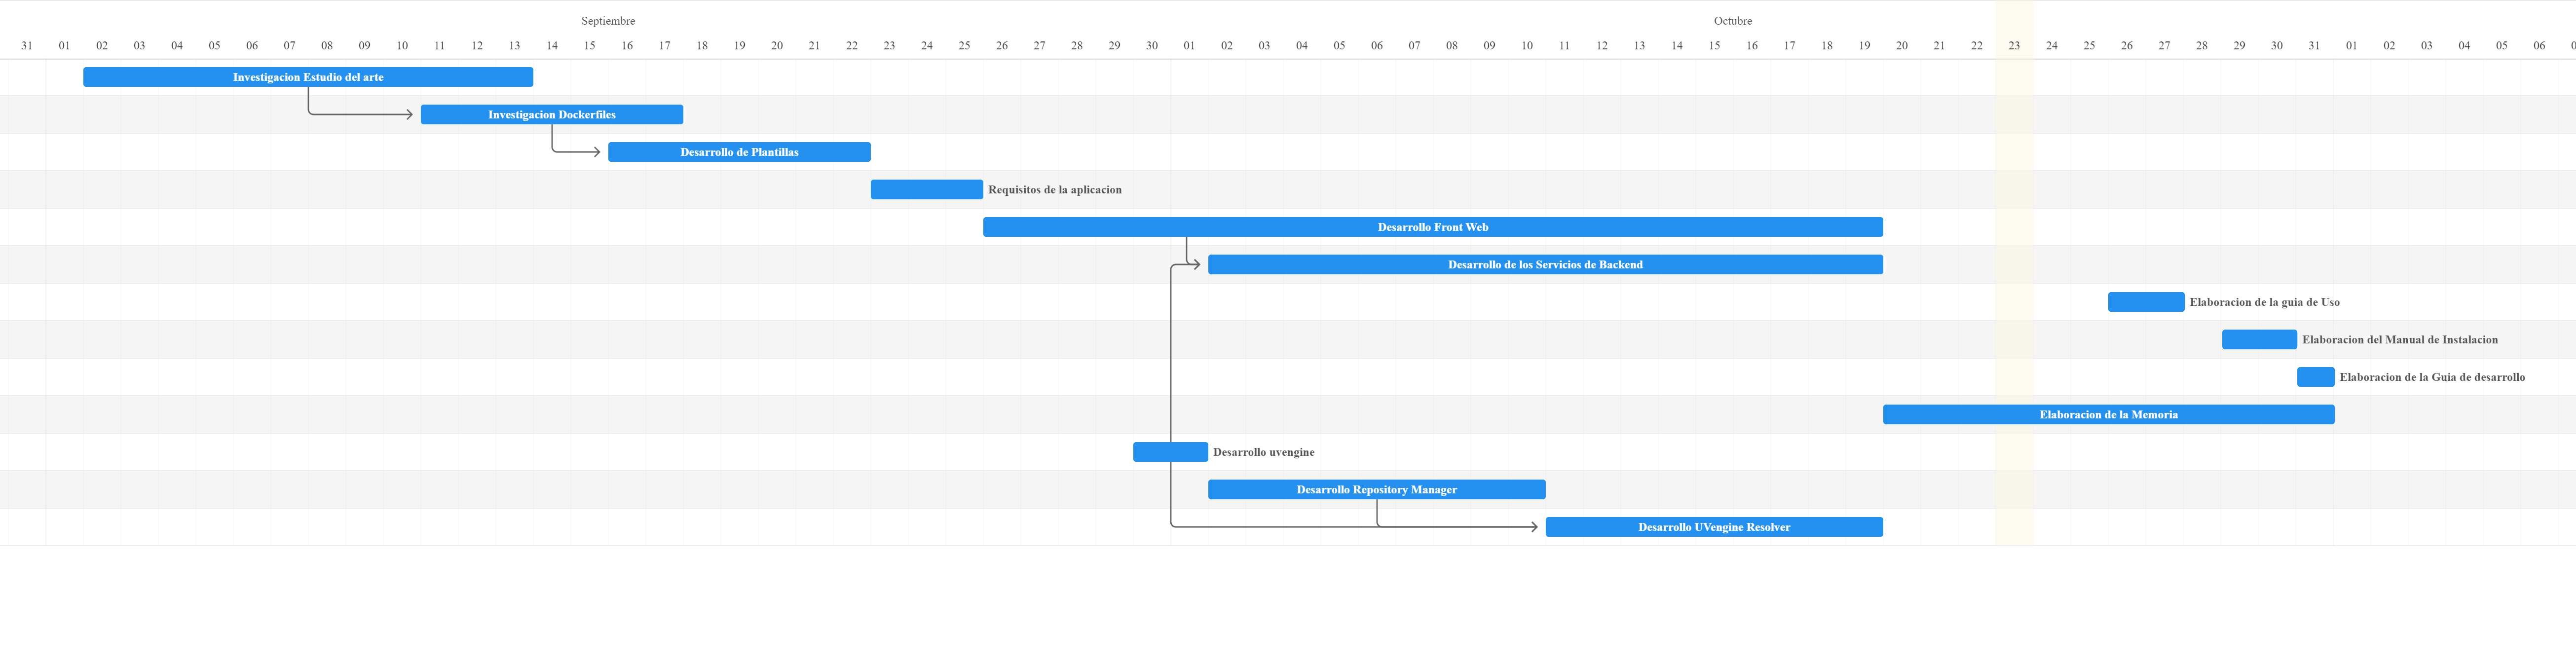
\includegraphics[width=1\textwidth]{gantt.png}
	\caption{Digrama de gantt} \footnote{Digrama generado por la herramienta https://www.plandemejora.com/crear-diagrama-de-gantt-online/}
\end{figure}
\subsubsection{Procedimiento}
Se evaluara con el tutor los momentos más relevates como los requititos de la aplicacion, Arquitectura y una evaluacion final para introduccir cambios que resulten necesarios en tanto en el proyecto como 
en la documentacion.

\subsubsection{Limitaciones}
El desarrollo de un proyecto de estas características requiere de una planificación y una metodología de trabajo adecuada.
En este sentido, como se han identificado anteriormente una serie de limitaciones y restricciones que pueden afectar al desarrollo del proyecto.
para el caso el desarrollo de las plantillas tiene que verse limitado en cuanto a formato y contenido, ya que no se puede abarcar todas las posibles opciones de configuracion.
\\El tiempo que se puede dedicar al proyecto tiene que estar dentro de unos limites razonables para un trabajo de estas caracteristicas y no se puede extender indefinidamente.

\subsection{Fases de Estudio}

\subsection{Estudio del Estado del Arte :}
En esta fase se realiza una revisión exhaustiva de la literatura y tecnologías existentes relacionadas con el tema del 
proyecto. El objetivo es comprender el panorama actual, identificar tendencias, mejores prácticas y tecnologías 
relevantes que puedan influir en el desarrollo del proyecto. Los puntos clave de esta fase son:

\begin{itemize}
	\item Para comprender la tecnologia de los contenedores fue exencial la lectura de \href{https://www.oreilly.com/library/view/docker-certified-associate/9781839211898/c5ecd7bc-b7ed-4303-89a8-e487c6a220ed.xhtml#uuid-1a5da664-fb76-4e56-bdb0-83255dde9e78}{Modern Infrastructures and Applications with Docker} \cite{docker_certified_associate}
	\item Completar la intruduccion al lenguaje uvl con \href{https://uvl.uni-ulm.de/}{UVL Playground} \cite{uvl_playground}
\end{itemize}

\subsection{Investigación diseño de dockerfiles}
Esta fase implica investigar y evaluar las diferentes opciones de configuracion que se presentan en el desarrollo de un fichero dockerfile en el 
despliegue de aplicaciones. Se exploran las características, herramientas y técnicas que pueden optimizar el uso de 
Docker en un proyecto software. 

\begin{itemize}
	\item Para compreder la importacia de las buenas practicas en la creacion de imagenes fue necesario la lectura de la documentacion oficial de Docker \href{https://docs.docker.com/reference/dockerfile/}{Dockerfile reference} \cite{dockerfile_reference}
\end{itemize}

Es necesario conocer como se aplica a la practica la creacion de imagenes. para ello han estudiado entre otros los siguientes proyectos:


\subsection{Desarrollo de Plantillas}
Esta fase implica la construcción el árbol de características y las restricciones textuales que orienten el espacio de 
configuraciones posibles del fichero Dockerfile. En este paso se pondran en practica todo el conocimiento adquirido en los pasos anteriores que 
tendran como resultado el modelado de unas plantillas. Hemos de tener en cuenta las buenas practicas y las recomendaciones de la comunidad para la creacion de los ficheros dockerfile \cite{dockerfile_concepts}. 
Estas practicas tienes que estar presentes en el diseño de las plantillas desde el inicio, tambien hemos de generar test para mantener la consistencia de las implementaciones. 
Esta fase queda cubierta con más detalle en el \hyperref[sec:Modelado de las plantillas]{Capitulo 5}.


\subsection{Fase Implementacion Cascada}
\subsubsection{Requisitios de la aplicación }
Aquí se definen y documentan los requisitos funcionales y no funcionales de la aplicación. Se recopilan y analizan las 
necesidades de los posibles usos, los objetivos del proyecto y las restricciones técnicas para establecer una planificacon del desarrollo. 
Los requisitos han cambiado conforme el proyecto avanzaba en sus etapas de desarrollo
sin animo de ser exhaustivos las funcionalidades mínimas que se pretenden alcazar son en cuanto a la generacion de productos.
\begin{itemize}
	\item La aplicacion web debe permitir seleccionar la plantilla y la version con la que se desea trabajar 
	\item Las plantillas pueden recargarse del repositorio 
	\item La aplicacion web debe generar un el producto en el momento en el que se aplique una configuracion valida 
\end{itemize}

\subsubsection{Desarrollo del Paquete uvengine }
En esta fase se adapta el proyecto de la aplicación de uvengine \cite{uvengine_github}, que permite la generación automática de archivos de configuración.
La adaptacion consiste en hacer opcional el fichero mapping model REFERENCIA a la hora de generar un producto, una vez adaptado se procede a la creacion de un paquete de python que se pueda instalar en cualquier entorno de desarrollo.
como resultado tenemos el paquete uvengine \cite{uvengine_pypi} \footnote{El paquete es empleado en el proyecto UVEngine-Resolver y en los entornos de desarrollo de las plantillas}
\subsubsection{Desarrollo Frontend de la web}
En esta fase se desarrolla la aplicación web que permite la interacción con el usuario y la visualización de los archivos de configuración generados.
La idea fundamental es permitir al usuario elegir entre un abanico de plantillas y versiones para que pueda decidir que producto generar en base a la configuracion que se aporte como entrada.
Debe funcionar como una abstraccion de los servicios de Backend para permitir al usuario trabajar desde una interfaz web.
\subsubsection{Desarrollo de los servicios de backend}
En esta fase se desarrollan los servicios de backend que permiten la comunicación entre la aplicación web y la aplicación de uvengine y los repositorios.
\subsubsection{Elaboración de la guía de uso}
En esta fase se elabora una guía de uso que explica cómo utilizar la aplicación y las funcionalidades disponibles.
Se elabora una guía detallada que describe cómo utilizar la aplicación, incluyendo instrucciones paso a paso, capturas 
de pantalla y ejemplos. 
\subsubsection{Elaboración de un manual de instalación}
En esta fase se elabora un manual de instalación que explica cómo instalar y configurar la aplicación en un entorno local.
\subsubsection{Elaboración de un manual de desarrollo de plantillas}
En esta fase se elabora un manual de desarrollo de plantillas que explica cómo crear y mantener plantillas para la aplicación.
\subsection{Elaboración de la memoria}
En esta fase se redacta la memoria o informe final del proyecto, que documenta todo el proceso de desarrollo, desde la 
planificación hasta la implementación y las lecciones aprendidas. La memoria incluirá el análisis de los resultados, 
conclusiones y recomendaciones para trabajos futuros. 



















%% Modelado de las plantillas
\section{Modelado de las plantillas}
\label{sec:Modelado de las plantillas}
Este espacio pretende describir de forma detallada el modelado de las plantillas y a que necesidad responden en la contruccion de un fichero de configuracion
\subsection{Introducción}
Dar cabida a la gran cantidad escenarios y posibles caso de uso para la apliacion se ha descrito anteriormente como una tarea abrumadora.
Aunque pudieramos crear una plantilla lo suficientemente expresiva para dar cabida a todos los escenarios de uso exitentes hasta la fecha, las plantillas quedarian desfasadas conforme se suceden cambios 
en las metodologias, surgen nuevas imagenes base, otras quedan desactualizadas etc. La obra resultante llegaria a ser inpracticable en cuanto a la cantidad de opciones y configuraciones que se podrian dar.
El objetivo del desarrollo todas las plantillas de este proyecto no pretende llegar a un nivel extremadamente avanzado de personalizacion, sino que sirvan como base para la creacion de plantillas más especificas y detalladas.

\subsection{Componentes de las plantillas}
Las plantillas se dividen en varios componentes 
\subsubsection{Featuremodel(.uvl)}
El archivo uvl es el archivo principal de la plantilla, contiene la descripcion de las caracteristicas y las restricciones de la plantilla.
en este archivo dicta principalmente como se generera una configuracion valida que sea capaz de cumplir con las restricciones textuales IMAGEN  CITA 
\subsubsection{Plantillas Jinja}
Las plantillas Jinja son los archivos de plantilla que se utilizan para generar los productos a partir de una configuracion valida o no del modelo. CITA
La idea es exponer estas plantillas ante una configuracion ya validadada con herramientas como UVLS CITA, Estas plantillas constituyen el nuecleo del funcionamiento, en ella se declaran de forma explicita las opciones de configuracion y las variables que se pueden modificar.
Las plantillas tienen que tener la esctrutura necesaria como para Usando la Sintaxis de Jinja crear un producto valido para una configuracion existente
\subsubsection{Mapping Model}
Es el unico componente completamente Opcional IMAGEN
Contiene la extructura de un fichero csv de tres con columnas. Las primeras columnas permiten mapear features sean estas booleanas o no a otros feature Boolenas que podran ser empleadas en las plantillas jinja, la tercera columna permite especificar una feature
Este archivo permite renombrar features y hacerlas más comprensibles para las plantillas jinja. Tambien es el responsable de hacer funciar configuraciones sobre otras plantillas.
\subsection{Plantilla dockerfile}
Como hemos visto un fichero Dockefile es un archivo de texto que contiene una serie de instrucciones que Docker CITA utilizará para construir una imagen de contenedor.
la plantilla para dockerfile cuenta con el modelo más grande del proyecto, La idea para crear estos modelso es subdividir el modelo en partes más pequeñas y manejables, de forma que se pueda trabajar con ellas de forma independiente.
El criterio a la hora de hacer subdivisiones es similar al criterio que usan repositorios como Docker HUB CITA donde divide sus imagenes por categorias dependiendo de su funcion.
En este contexto podemos construir una primera subdivision que represente el resultado final esperado, es decir la primera feature sera decidir si nuestra imagen 
tiene el objetivo de desplegar un contenedor que albergue un Frontend, Backend, Base de datos, etc.
\begin{figure}[ht]
	\centering
	  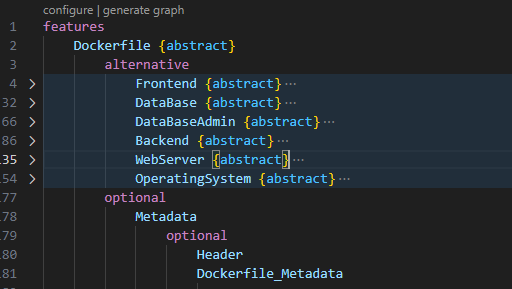
\includegraphics[width=0.5\textwidth]{dockerfile.uvl.png}
	\caption{Captura de la primera subdivision para dockerfile.}
\end{figure}

Cada una de estas categorias contendra a su vez una serie de subcategorias que representen las opciones de configuracion que se pueden dar en cada una de ellas.
Centremonos en el caso de uso de un Frontend, Comunmente al deplegar una imagen de frontend se sigue una estrategia de multi etapa CITA donde en una primera etapa compilamos la aplicacion 
y en una posterior etapa la alojamos en un servidor web, esto con el objetivo de crear una imagen lo más pequeña posible al no contener ninguno de los ficheros fuente

en este caso las subcategorias podrian ser el lenguaje, el puerto en el que se desplegara la aplicacion, el comando que se ejecutara al iniciar el contenedor, etc.
Estos son elementos ya mecionados en la seccion de herramientas disponibles como pueden ser Docker Init CITA, Nuestro modelo permite recojer estas caracteristicas además de otras 
como pueden ser el servidor web que queremos junto con su version, Podremos seleccionar el framework de desarrollo que se ha empleado, la version en la que compilara la aplicacion etc.
Las posibilidades van mucho más alla de lo que se recoje en esta version del fichero dockerfile pero estas opciones ya expanden enormemente la capacidad de configuracion que tienen otras 
herremientas. 
  
\begin{figure}[ht]
	\centering
	  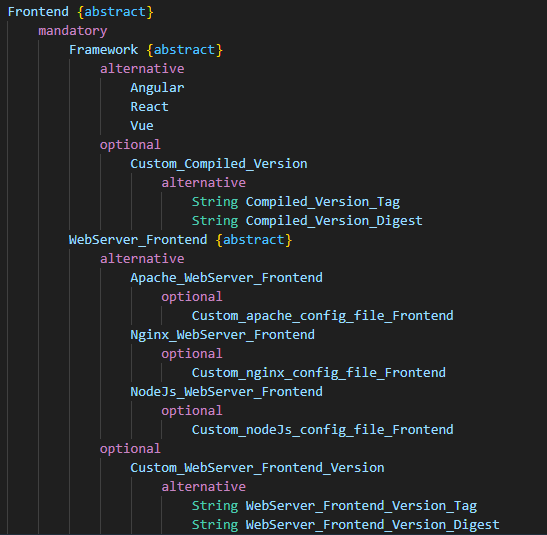
\includegraphics[width=0.5\textwidth]{dockerfile.frontend.png}
	\caption{Captura de la primera subdivision para dockerfile.}
\end{figure}

\subsubsection{Plantillas Jinja2}
Una vez que contamos con el modelo de la plantilla, podemos proceder a la creacion de las plantillas Jinja2 que son quienes realmente aportan el contenido al producto.
La sintaxis de Jinja2 nos permite aplicar cierta lógica a la hora de generar los ficheros de configuracion, por ejemplo podemos emplear condicionales para que ciertas partes del fichero se generen o no en funcion de la configuracion que se haya dado.
Dividir las plantillas no solo es util porque las hace más manejables y faciles de mantener, sino que tambien permite la reutilizacion de las mismas, por ejemplo si tenemos una plantilla que se repite en varias plantillas, podemos extraerla a un fichero aparte y reutilizarla en todas las plantillas que lo necesiten.
Para este caso podemos generar una plantilla para los metadatos y labels de la imagen 

\begin{figure}[ht]
	\centering
	  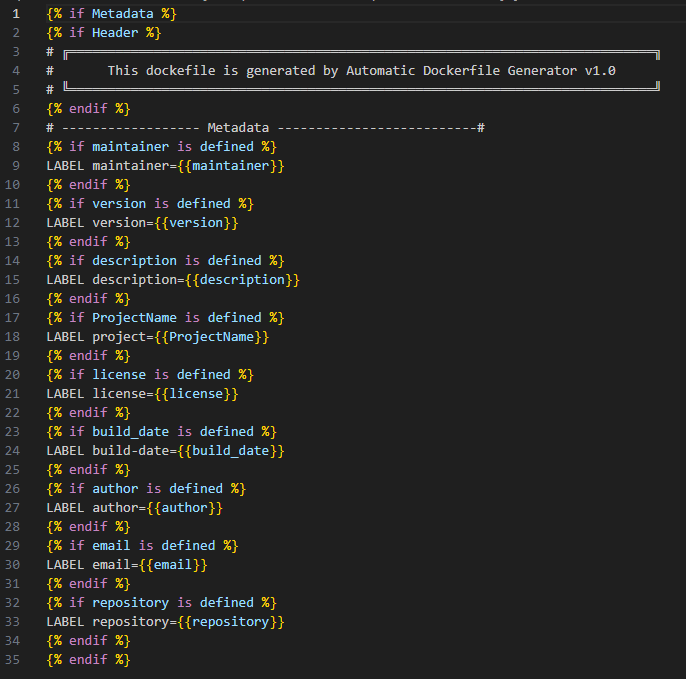
\includegraphics[width=0.5\textwidth]{dockerfile.metadata.png}
	\caption{Captura de la primera subdivision para dockerfile.}
\end{figure}

\begin{figure}[ht]
	\centering
	  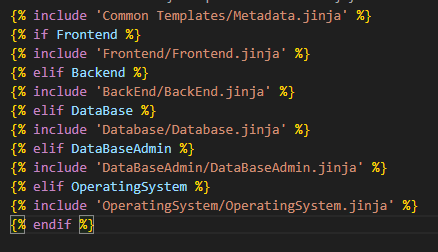
\includegraphics[width=0.5\textwidth]{dockerfile.logica.plantillas.jinja.png}
	\caption{Captura de la primera subdivision para dockerfile.}
\end{figure}

\begin{figure}[ht]
	\centering
	  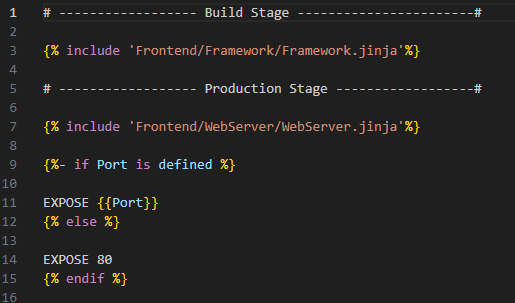
\includegraphics[width=0.5\textwidth]{dockerfile.frontend.jinja.template.png}
	\caption{Captura de la primera subdivision para dockerfile.}
\end{figure}

\subsubsection{Test sobre la Plantilla dockerfile}
El diseño y construccion de las plantillas es un proceso incremental, debe comprobarse con regularidad si nuestra intencion a la hora de seguir desarrollar una plantilla es mantener 
una coherencia con lo añadido hasta el momento. Con esta idea en mente la solucion propuesta consiste en la creacion de pruebas que validen la correcta construccion de productos segun la plantilla en la que estamos trabajado.
Estas pruebas deben ser capaces de comprobar que las plantillas generan un producto correcto. para el caso del dockerfile estas pruebas deben componerse por cada configuracion 
y un producto esperado, si nuetra plantilla es capaz dada lo configuracion de entrada generar el mismo producto la prueba sera considerada como exitosa. 

\newpage

\begin{figure}[ht]
	\centering
	  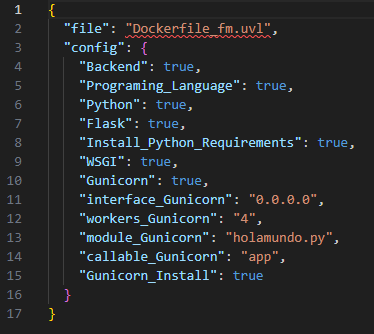
\includegraphics[width=0.5\textwidth]{dockerfile.configuracion-backend.png}
	\caption{Conguracion Ejemplo 1 Backend.}
\end{figure}

\begin{figure}[ht]
	\centering
	  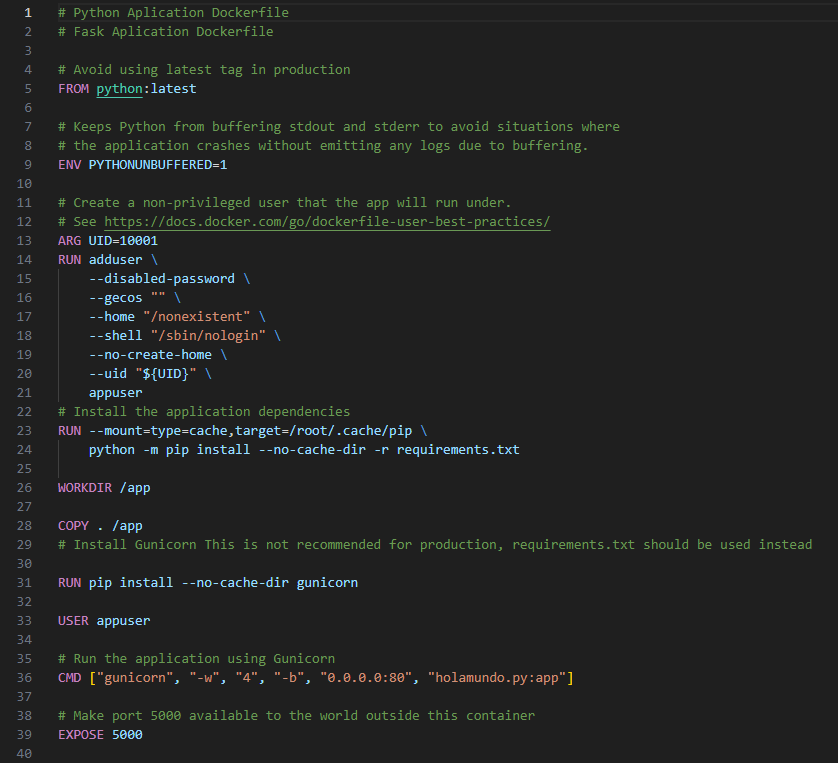
\includegraphics[width=1\textwidth]{dockerfile.backend.producto.png}
	\caption{Producto Esperado.}
\end{figure}

\newpage

es evidente que ciertos cambios más radicales plantean refactorizar algunos test. aun asi es aconsejable validar el diseño de los nuevos elementos de la plantilla solucionando estas incoherencias.
En el contexto de esta plantilla dockerfile las pruebas se han realizado empleado las librerias de pytest CITA para la generacion de los productos esperados.
para cada una de las primeras divisiones de las plantillas se generan ficheros de test para clasificar las configuraciones que se prueban y los productos esperados.


\begin{figure}[ht]
	\centering
	  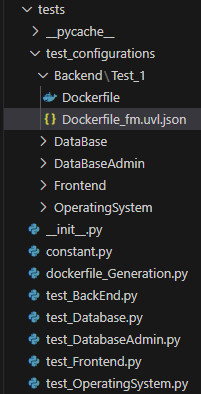
\includegraphics[width=0.2\textwidth]{organizacion.test.pytest.png}
	\caption{Captura de la primera subdivision para dockerfile.}
\end{figure}




















%% Arquitectura y Descripcion del sistema
\section{Arquitectura y Descripcion del sistema }
\label{sec:Arquitectura y Descripcion del sistema}
Esta seccion describe la arquitectura y el modelado del sistema, incluyendo los componentes, la estructura y el diseño de la aplicación resultante.
\subsection{Vision general de la arquitectura }
La arquitectura de la aplicación se divide en dos partes principales: el backend y el frontend.
El backend es responsable de la generación de los archivos de configuración a partir de las plantillas y de la comunicación con los repositorios de plantillas.
El frontend es responsable de la interacción con el usuario y la visualización de los archivos de configuración generados.
\subsection{Descripcion de servicios de backend}
Para los servicios de backend estos se han dividido en varios servicios que se encargan de tareas especificas.
La primera de ellos es Repository Manager CITA este servicio se encarga de servir traducir las peticiones que puede realizar el front end a la API de GitHub.
Estas peticiones son descargar el archivo uvl de la plantilla y version seleccionada, descargar el listado de plantillas disponibles y descargar el listado de versiones disponibles para cada plantilla
\subsubsection{Repository Manager}
Esta aplicaicon esta desarrollada en Python y emplea el framework Flask para la creacion de la API, esta API se encarga de servir los archivos uvl de las plantillas y las versiones disponibles.
para hacer funcionar esta API se emplea la api publica de github que permite acceder al contenido de repositorios. 
En este caso el repositorio al que queremos acceder es el repositorio Templates CITA que contiene las plantillas disponibles.
\subsubsection{UVEngine Resolver}

La segunda de ellas es UV Engine Resolver CITA este servicio se encarga de resolver la variabilidad a partir de recibir como parametros Un fichero Json que contiene el nombre de la plantilla, la version a utilizar y la configuracion 
el resultado de la funcion sera un producto
\subsection{Descripcion de Frontend}



%% Extesivilidad de la aplicación
\section{Extensibilidad}
\label{sec:Extensibilidad}
En esta seccion se pretende hacer incape en la extensibilidad de la aplicacion, como se ha mencionado anteriormente el proyecto tiene en mente que pueda adaptarse a las necesidades futuras.

Al almacernar las plantillas en un repositorio publico de GitHub, se permite a cualquier usuario modificar, añadir o eliminar plantillas de forma sencilla.
Esot permite que el desarrollo de plantillas se maneje de forma independiente al resto de la aplicacion y que se puedan añadir nuevas plantillas sin necesidad de modificar el codigo de la aplicacion.
\subsection{Añadir Plantillas}
Existiendo varias formas en las que se pudiera haber diseñado la forma con la que añadir nuevas plantillas a la aplicacion aprovechando caracteristicas de Github se ha optado por la solucion más sencilla y directa.
Añadir una nueva plantilla es tan sencillo como añadir una nueva carpeta al repositorio de plantillas de GitHub.
Esta carpeta debe contener una estructura de directorios especifica que contenga los archivos necesarios para la plantilla como son el archivo uvl, las plantillas Jinja2 y el archivo de Mapping Model, este ultimo archivo es opcional.
Existen instucciones detalladas de como añadir una plantilla al respositorio de plantillas en CITA 

\subsubsection{Ampliar la Plantilla Dockerfile}
La Plantilla Dockerfile recoje alguna de las caracteristicas más interesantes que ya cubren otras herramientas pero queda claro que todavia existe mucho margen de mejora en cuanto a la personalizacion de las opciones de configuracion.
La plantilla no es a dia de hoy capaz de cubrir todas las opciones de configuracion que se pueden dar en un fichero Dockerfile, pero tiene el potencial de ser ampliada y mejorada en el futuro.
Ampliar esta plantilla es sencillo, se cuenta ya con un repositorio de desarrollo para la plantilla CITA que contiene la plantilla y los test necesarios para validarla.
Una vez que se haya ampliado la plantilla, se puede añadir al repositorio de plantillas de GitHub y utilizarla para generar productos.











%% Despliegue de la aplicación
\section{Despliegue de la aplicación }
\label{sec:Despliegue de la aplicación}
\subsection{ Despliegue local }
Para desplegar el proyecto y todas sus capas se hace uso de la herramienta Docker CITA, que permite la creación de contenedores ligeros y portables que pueden ejecutarse en cualquier entorno.
Para el despliegue local se hace uso de Docker Compose CITA, que permite definir y ejecutar aplicaciones Docker multi-contenedor generando todos los servicios necesarios para el despliegue de la aplicación.
Esto supone una abstracción de la infraestructura necesaria para el despliegue de la aplicación, permitiendo la creación de un entorno de desarrollo y pruebas aislado y reproducible.
En el proyecto se encuentra el fichero docker-compose.yml que contiene la configuración necesaria para el despliegue de la aplicación en un entorno local.
\begin{verbatim}
	version: '3.8'

	services:
	  fronted:
		build:
		  context: ./Frontend
		  dockerfile: dockerfile
		container_name: frontend
		ports:
		  - "4200:80"
	  
	  repository-manager:
		build:
		  context: ./Repository-Manager
		  dockerfile: dockerfile
		container_name: repository-manager
		ports:
		  - "5000:5000"
	
	  uvengine-resolver:
		build:
		  context: ./UVEngine-Resolver
		  dockerfile: dockerfile
		container_name: uvengine-resolver
		ports:
		  - "5001:5001"
		depends_on:
		  - repository-manager
	  
	  nginx-reverse-proxy:
		build:
		  context: ./Nginx-Reverse-Proxy
		  dockerfile: dockerfile
		container_name: nginx-reverse-proxy
		ports:
		  - "80:80"
	\end{verbatim}

Como se observa el codigo se compone de 4 servicios 
\begin{itemize}
	\item Frontend: Servicio que se encarga de servir la aplicacion web
	\item Repository Manager: Servicio que se encarga de servir los archivos uvl de las plantillas y las versiones disponibles
	\item UVEngine Resolver: Servicio que se encarga de resolver la variabilidad a partir de recibir como parametros Un fichero Json que contiene el nombre de la plantilla, la version a utilizar y la configuracion 
	\item Nginx Reverse Proxy: Servicio que se encarga de redirigir las peticiones de la aplicacion web al servidor de backend y fronte	
\end{itemize}

La instruccion dockercompse up creara los contendores en la configuracion ya escrita. La web sera accesible en la direccion localhost en el puerto 80

\subsection{ Despliegue en la nube }
Por definir 





%% Resultados
\section{Resultados}
\label{sec:Resultados}
Esta parte del documento se centra en los resultados obtenidos durante el desarrollo del proyecto, incluyendo los resultados de las pruebas, la viabilidad del proyecto, y la escalabilidad.
\subsection{Resultados Obtenidos}
Cumpliendo los objetivos propuestos al inicio del proyecto, se ha desarrollado una aplicación que permite la generación automática de archivos de configuración a partir de plantillas.

Un resumen de los resultados del proyecto es el siguiente:

\begin{itemize}
\item La Plataforma web de la aplicacion aporta una forma agil de crear productos software a partir de ellas.

\item Las plantillas para generar ficheros como dockerfiles recogen una un interesante número de posibilidades entre las que se encuentran las opciones más usuadas
una vez generamos una configuracion podemos simplemente descargar el fichero generado o copiarlo al portapapeles y quedaria listo para su uso.

\item El empleo de la extension uvls para generar una configuracion puede ser muy eficiente a la hora de generar productos con opciones de configuracion relacionadas entre si
Ademas tenemos la posiblidad de editar el producto final antes de utilizarlo.

\item Las plantillas exitentes aportan unas funcionalidades interensates que pueden explotarse a la hora de genera productos como ficheros de Configuracion

\item El repositorio es facilmente ampliable para abarcar nuevas plantillas y desarrollar nuevas funcionalidades
\end{itemize}

\newpage 

Resumen de los desarrollos resultantes del proyecto:
\begin{itemize}
	\item Se ha desarrollado una aplicación web que permite la interacción con el usuario y la visualización de los archivos de configuración generados.
	\item Se adaptado el uso del proyecto uvengine que permite la generación automática de archivos de configuración a partir de plantillas adaptandola a las necesidades del proyecto.
	\item Se ha desarrollado una aplicación de Repository Manager que permite la comunicación con los repositorios de plantillas en GiHub CITA .
	\item Se ha desarrollado una aplicación de UVEngine Resolver que permite la resolución de la variabilidad a partir de una configuración.
	\item Se ha creado la plantilla para la generación de ficheros Dockerfile a partir de una configuración.
	\item Se ha desarrollado la plantilla auxiliares para ficheros de configuracion Nginx, dockerignore, etc.
	\item Se han desarrollado pruebas para validar la correcta construcción de los productos a partir de las plantillas dockerfile.
	\item Se ha aportado todo el código fuente y la documentación necesaria para la replicación del proyecto.
	\item Se ha generado una Memoria que documenta todo el proceso de desarrollo.
	\item Se ha aportado apendices para el uso más fundamental de la aplicacion.
\end{itemize}

\subsection{Viabilidad del proyecto}
Como hemos recogido arriba el proyecto es potencialmente viable pero presenta algunas carencias que pueden ser corregidas.
Es posible que el uso mandatorio de la extension uvls para generar los ficheros de configuracion sea un punto en contra para la viabilidad del proyecto, pese a que la extension es un proyecto de codigo abierto y seria posible su integracion en la aplicacion.
Las soluciones actualmente actualemente disponibles son más comodas al detectar las features CITA del proyecto de forma autonoma sin necesidad de intervencion del usuario. Esto supone que esta solucion quede atras en cuanto a comodidad. Es conveniente que adaptar este sistema 
para que sea capaz de detectar algunas de las features de forma autonoma y dejar otras para la personalizacion del usuario al menos en cuanto nos referimos a la generacion del fichero dockerfile.
\subsection{Escalabilidad}
Teniendo en cuenta que la escalabilidad de cualquier aplicacion depende en la capacidad de sus servicios de generar nuevas instacias es en un principio viable 
escalar horizontalmente cada uno de los servicios. Sin embargo la escalabilidad de la aplicacion se ve limitada actualmente por el uso de API publica de github CITA 
para el servicio de Repository manager CITA que limita el numero de peticiones que se pueden hacer en un periodo de tiempo.
\footnote{Actualmente el número de peticiones que puede realizarse a la api son 80 peticiones por minuto CITA esto es propenso a que cambien en un futuro.}
En el escenario en el que se quiera llevar la aplicacion a un entorno de produccion debe sortearse este problema bien por medio del uso de tokens de autenticacion.
Existe la posbilidad de que el usario aporte un token personal de una cuenta de gitHub a la hora de desplegar el servicio o bien emplear un token propio desde Github.

En el escenario de superar dicho limite desde la aplicacion no se podra descargar modelos uvl ni se podra recargar el listado de plantillas y ni versiones de las mismas.
No obstante se podra resolver la variabilidad de las plantillas que ya se han descargado y se podra generar productos a partir de ellas si se encuentran disponibles en los servicios 
uvengine-resolver CITA 









%% Conclusiones
\section{Conclusiones y líneas Futuras }
\label{sec:Conclusiones}


\subsection{Conclusiones del Desarrollo del proyecto}
El desarrollo del proyecto ha permitido alcanzar los objetivos planteados inicialmente. Se ha logrado implementar una solución eficiente y potencialmente escalable que cumple con los requisitos funcionales y no funcionales establecidos. Además, se ha adquirido un conocimiento profundo sobre las tecnologías utilizadas y se han identificado áreas de mejora para futuros desarrollos.
El desarrollo de las plantillas ha sido conservador y no se ha considerado explorar más que casos basicos de uso. Esto era algo esperado si asumimos la gran casuistica que tenemos, sin embargo se ha demostrado que la aplicacion es capaz de generar productos validos a partir de configuraciones validas. Dado el nivel de desarollo de las herramientas (uvls) y tecnologias de las que hace uso este proyecto se ha demostrado que es posible llevar a cabo un proyecto de estas caracteristicas.
\subsection{Conclusion Personal}
A nivel personal, el desarrollo de este proyecto me ha servido para introduccirme de lleno en la tecnologia de contenedores, como esta tecnologia se aplica en servicios y que implicaciones existen a nivel de rendimiento y seguridad. Considero que el proyecto tiene de base una serie de fortalezas que otra serie de herramientas no consigue ofrecer actualmente. Es posible que un proyecto más ambicioso y con más recursos pueda explotar estas fortalezas y llevar el diseño de productos por este camino.
Sin duda el proyecto queda lejos de tener aplicaciones funcionales reales pero muestra un camino que puede ser explotado si se considera. 
\subsection{Aplicaciones Prácticas}
Ademas de contar con una forma intersante de generar dockerfiles pueden existir dinamicas para aprovechar configuraciones validas para generar otros ficheros necesarios, como por ejemplo podemos ficheros de configuracion para el servidor de Nginx CITA directamente a partir de la configuracion para generar un dockerfile. Esto es gracias a los ficheros Mapping Models y a un diseño inteligente de las plantillas
\subsection{Desarrollo de nuevas plantillas }
El proyecto esta preparado para recibir nuevas plantillas no solo para la generacion de ficheros dockerfile y algunos de los archivos de configuracion sino que se puede extender a otros tipos de ficheros, como por ejemplo ficheros de configuracion de Kubernetes CITA, ficheros de configuracion de Jenkins CITA, etc.
Una vez añadidas plantillas al repositorio estan estaran disponibles de la misma forma en la que estan disponibles las plantillas existentes solo sera necesario recargar el listado de plantillas que se encuentra en el la barra de navegacion de la aplicacion web.
\subsection{Continuación en el desarrollo de plantillas ya existentes}
Las plantillas exitentes tienen un gran margen de mejora, En la situacion actual no soportan la gran mayoria de las opciones de configuracion que se pueden dar en un fichero Dockerfile. Además las opciones que se manejar son propensas a quedar obsoletas y se necesita de una continua revision de las plantillas en busca de problemas de diseño o seguridad.

\subsection{Mejorar la experiencia del usuario }
La generacion de la configuraciones estan ligadas al desarrollo de la extension uvls, la extension permite al usuario generar una configuracion valida deplegando el arbol de caracteristicas CITA pero para ello el usuario
necesita contar con VSCode y la extension instalada. para ser capaz de generar configuraciones validas. La propuesta para este escenario seria la integracion de dicha funcionalidad dentro de la plantaforma web,
la extension uvls es un proyecto de codigo abierto y su integracion en la aplicacion web podria ser un proyecto en si mismo. 

En el desarrollo del trabajo se ha explorado esta posibiliddad ejecutando dicha extension en la version
web del editor VS code pero el resultado en cuanto a rendimiento hace que esta opcion no sea viable.

La propia aplicacion web puede ser mejorada en cuanto a la experiencia del usuario añadiendo más informacion al usuario para colocar más contexto a la hora de seleccionar una plantilla y las posiblidades de combianar configuraciones 







%%%% Sections
%%\section{One \\}
%%
%%\subsection{Motivation}
%%    \blindtext[2]
%%    
%%    \begin{figure}[ht]
%%      \centering
%%        
\includegraphics[width=0.5\textwidth]{xp}
%%      \caption{A diagram showing the iterations of extreme programming.}
%%    \end{figure}
%%    
%%    \blindtext[4]
%%
%%\section{Two \\}
%%    \blindmathpaper






% Imprimir la bibliografía
\printbibliography




%% Bibliografia
%%\begin{thebibliography}{9}
%%    \bibitem{latexcompanion} 
%%    Michel Goossens, Frank Mittelbach, and Alexander Samarin. 
%%    \textit{The \LaTeX\ Companion}. 
%%    Addison-Wesley, Reading, Massachusetts, 1993.
%%    
%%    \bibitem{einstein} 
%%    Albert Einstein. 
%%    \textit{Zur Elektrodynamik bewegter K{\"o}rper}. (German) 
%%    [\textit{On the electrodynamics of moving bodies}]. 
%%    Annalen der Physik, 322(10):891–921, 1905.
%%\end{thebibliography}




%%\end{document}















%% Apendices

\begin{umaappendices}
    \section{Manual de \\ Instalación}
	\label{sec:Manual de Instalación}
	\subsection{Requisitos Previos}
	\subsection{Descargar el codigo fuente}
	\subsection{Configuracion del archivo Dockercomose}
	\subsubsection{Nginx reverse proxy}
	\subsubsection{frontend}
	\subsubsection{Repository Manager}
	\subsubsection{UV Engine resolver}
	\subsection{Construccion de los contenedores}
	\subsubsection{Github API}
	\subsection{Terminar el servicio}



    \section{Manual de Uso}
	\label{sec:Manual de Uso}
	\subsection{Inicio de la aplicacion}
	\subsection{Barra de Navegación}
	\subsubsection{About Page}
	\subsubsection{Help Page}
	\subsection{Seleccionar plantilla}
	\subsubsection{Seleccionar version de la platilla}
	\subsubsection{Cargar configuracion}
	\subsubsection{Descargar Fichero Generado}
	\subsubsection{Copiar Fichero Generado}




	\section{Manual de Desarrollo}
	\label{sec:Manual de Desarrollo}
	\subsection{Manual de Desarrollo de Plantillas}
	\subsubsection{Como añadir nuevas plantillas al repositorio}
	\subsubsection{Como modificar las plantillas del repositorio}




\end{umaappendices}


%% Back Cover

\includepdf[noautoscale=true, width=\paperwidth]{Portada-Titulo-Contraportada/backcover.pdf}
\end{document}



\end{document}